\subsection{WebsocketServer}
\begin{figure}[ht]
  \centering
  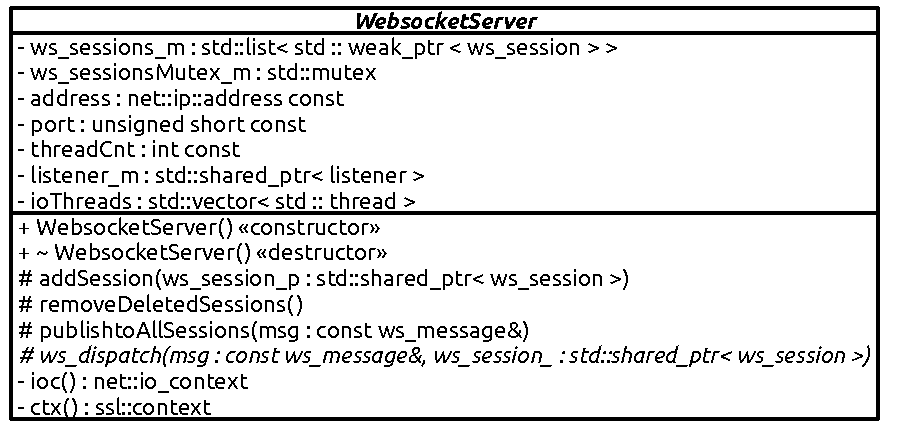
\includegraphics[width=\textwidth]{content/hauptteil/umsetzungPoC/backend/uml/classesOfOverview/WebsocketServer.pdf}
  \caption{Klassendiagramm der Klasse \eigenName{WebsocketServer}}
  \label{fig:backend:classDiag:WebsocketServer}
\end{figure}
Die Klasse \eigenName{WebsocketServer} (\refFig{fig:backend:classDiag:WebsocketServer}) verwaltet die offenen Websocket Sessions (Objekte der Klasse \eigenName{ws\_session}).
Sie bedient sich dabei der bekannten  C++ Bibliothek \eigenName{Boost.Beast} \citep{beast:lib}.
Websocket Sessions sind die einzelnen Verbindungen zwischen Backend und Frontend.
Das Aufbauen von Verbindungen ist den Beispielen von Vinnie Falco zur \eigenName{Boost.Beast} Bibliothek entnommen \citep{beast:examples}.
Die \eigenName{WebsocketServer} Klasse speichert dabei, pro aktiver Websocket Session, einen Pointer des zugehörigen \eigenName{ws\_session} Objekts in einer Liste.
Diese Liste existiert als das Attribut \eigenName{ws\_sessions\_m} in der Klasse \eigenName{WebsocketServer} und ist zusätzlich durch ein Mutex geschützt.
Diese Mutex kann man sich vorstellen wie ein Schloss, das immer zuerst gesperrt werden muss, 
bevor die Session Liste verfügbar ist (Aufruf von \eigenName{std::mutex::lock()}). 
Ist das Mutex von einem Thread gesperrt, so kann ein anderer Thread es solange nicht sperren wie es noch gesperrt ist.
Damit wird der zeitgleiche Zugriff von mehreren Threads auf eine Datenstruktur verhindert (Race Conditions werden verhindert).
Wäre das nicht der Fall könnte es beispielsweise passieren dass ein Element gleichzeitig gelöscht wird, während ein anderer Thread lesend auf das Element zugreift.
Solche Race Conditions bedarfen keiner echten Simultanität (mehrere Prozessorkerne die auf den selben Speicherbereich zugreifen), sie können auch durch das Scheduling des Betriebssystem entstehen. 
Ist ein Thread nun mit der Arbeit an der geschützten Ressource fertig, gibt er sie wieder frei indem er die Methode \eigenName{std::mutex::unlock()} aufruft.
Das scheint der einfachste Weg zu sein, aber nicht der sicherste. 
Wenn im Code zwischen \eigenName{lock()} und \eigenName{unlock()} eine Exception eintritt, 
wird zwar die Ressource danach nichtmehr benötigt, es wird aber auch nicht \eigenName{unlock()} aufgerufen.
Man spricht in diesem Fall von einem \emph{Deadlock}, da das Mutex von einem Thread gesperrt wurde und nie wieder entsperrt wird. 
Das führt dazu, dass alle anderen Threads, die die Ressource benötigen, endlos auf deren Freigabe warten. 
Um das zu verhindern bietet die \ac{stl} eine \eigenName{lock\_guard} Klasse, die bei ihrer Zerstörung das Mutex selbständig wieder frei gibt.
Diese Vorgehensweise sieht man in \refList{list:addSession}, wenn der \eigenName{lock\_guard} in Zeile 354 nicht mehr im Scope ist, wird automatisch \eigenName{unlock()} aufgerufen.
\begin{listing}[ht]
  \inputminted[linenos=true,breaklines=true, firstline=348, lastline=354]{c++}{../Backend/WebsocketServer.cpp}
  \caption{Methode \eigenName{addSession} der Websocket Server Klasse}
  \label{list:addSession}
\end{listing}
\begin{figure}[ht]
  \centering
  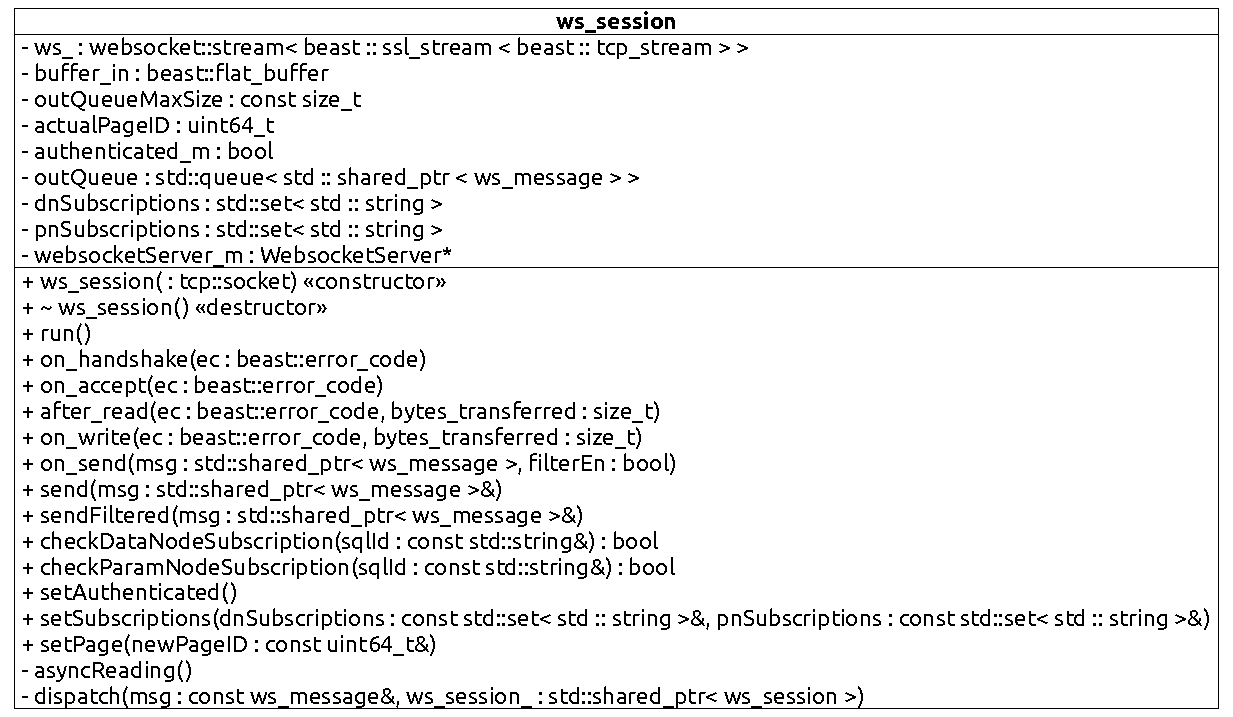
\includegraphics[width=\textwidth]{content/hauptteil/umsetzungPoC/backend/uml/classesOfOverview/ws_session.pdf}
  \caption{Klassendiagramm der Klasse \eigenName{ws\_session}}
  \label{fig:backend:classDiag:wsSession}
\end{figure}
Bei jeder neuen Websocket Verbindung wird ein neues \eigenName{ws\_session} Objekt (Klassendiagramm \refFig{fig:backend:classDiag:wsSession}) instanziert 
und bekommt dabei einen Pointer auf das \eigenName{WebsocketServer} Objekt. Dies ermöglicht dem \eigenName{ws\_session} Objekt 
sich bei dem \eigenName{WebsocketServer} Objekt anzumelden. 
Zusätzlich speichert das \eigenName{ws\_session} Objekt den Pointer unter dem Attribut \eigenName{websocketServer\_m} ab.
Dies ermöglicht es beim Empfang eines kodierten Strings durch das \eigenName{ws\_session} Objekt, ein \eigenName{ws\_message} Objekt aus dem String zu konstruieren
und die virtuelle Methode \eigenName{ws\_dispatch} der \eigenName{WebsocketServer} Klasse aufzurufen, welche in der \eigenName{Backend} Klasse reimplementiert wird.
Dort wird das \eigenName{ws\_message} Objekt dann entsprechend seines Events interpretiert und der entsprechende Handler (beschrieben in Abschnitt \ref{subsec:protokollBackendFrontend}, 
implementiert in der Methode \eigenName{ws\_dispatch}) ausgeführt.
Daten, die in die andere Richtung fließen, werden entweder direkt aus der Dispatcher Methode des Backends in eine einzelne Session geschickt (Aufruf der Methode \eigenName{send} des \eigenName{ws\_session} Objekts), 
oder über die Methode \eigenName{publishToAllSessions} der \eigenName{WebsocketServer} Klasse.
Dabei ist eine Art Publish/Subscribe Mechanismus implementiert, bei dem Änderungen die DataNodes oder ParamNodes betreffen nur dann über die jeweilige Websocket Session an das Frontend gesendet werden, 
wenn eine entsprechende Seite dargestellt ist, welche die Nodes auch verwendet.
\begin{figure}[ht]
  \centering
  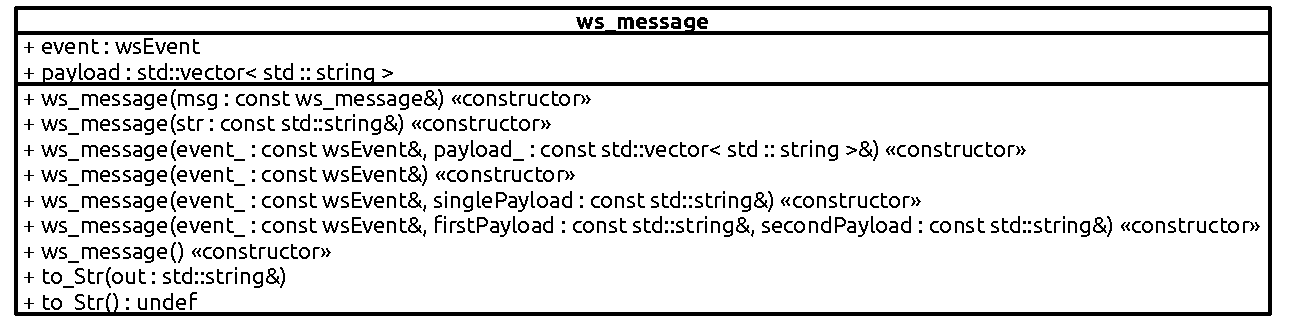
\includegraphics[width=\textwidth]{content/hauptteil/umsetzungPoC/backend/uml/classesOfOverview/ws_message.pdf}
  \caption{Klassediagramm der Klasse \eigenName{ws\_message}}
  \label{fig:backend:classDiag:wsMsg}
\end{figure}
Bei der Kommunikation mit dem Frontend werden, entsprechend des Abschnitts \ref{subsec:protokollBackendFrontend}, Strings ausgetauscht. 
Diese Strings werden beim Empfang in einem \eigenName{ws\_message} Objekt (Klassendiagramm in \refFig{fig:backend:classDiag:wsMsg}) gespeichert und zum Dispatcher transportiert. 
Dort kann dann auf die einzelnen Komponenten der Nachricht (Event und Payloadvektor) einzeln zugegriffen werden.
Außerdem ermöglicht die Klasse durch die Methode \eigenName{to\_Str} es ihren Inhalt wieder als String, zum Transport an das Frontend, zu kodieren.
Um den Code bei der Verwendung des \eigenName{ws\_message} Objekts so kurz wie möglich zu halten, stehen zum Konstruieren eine Vielzahl von Konstruktoren zur Verfügung.
